\chapter{Learning Roadmap}

Congratulations on finishing this guide! Where do you go from here?

\begin{figure}[H]
    \centering
    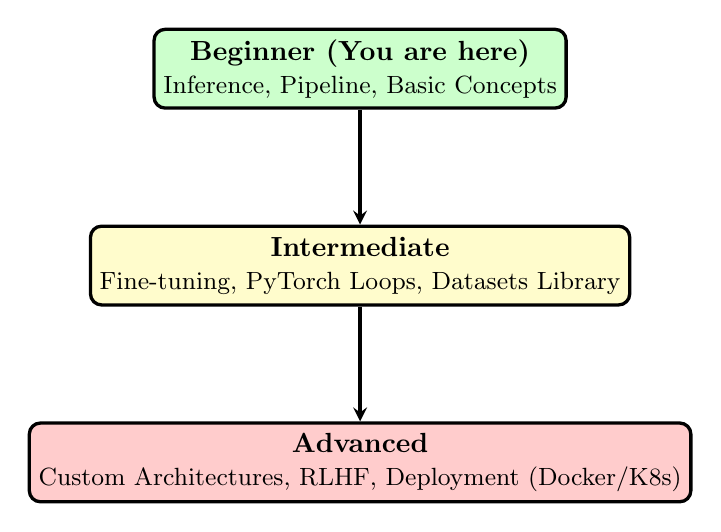
\begin{tikzpicture}[
        node distance=1.5cm,
        auto,
        level/.style={rectangle, draw=black, very thick, rounded corners, minimum width=3cm, minimum height=1cm, align=center},
        arrow/.style={->, >=stealth, very thick}
    ]
        \node[level, fill=green!20] (beginner) {\textbf{Beginner (You are here)} \\ \small Inference, Pipeline, Basic Concepts};
        \node[level, fill=yellow!20, below of=beginner, node distance=2.5cm] (intermediate) {\textbf{Intermediate} \\ \small Fine-tuning, PyTorch Loops, Datasets Library};
        \node[level, fill=red!20, below of=intermediate, node distance=2.5cm] (advanced) {\textbf{Advanced} \\ \small Custom Architectures, RLHF, Deployment (Docker/K8s)};

        \draw[arrow] (beginner) -- (intermediate);
        \draw[arrow] (intermediate) -- (advanced);
    \end{tikzpicture}
    \caption{Your Path Forward}
\end{figure}

\section{Recommended Resources}
\begin{itemize}
    \item \textbf{Hugging Face Course:} \url{https://huggingface.co/course} (The Bible of HF).
    \item \textbf{Fast.ai:} Practical Deep Learning for Coders.
    \item \textbf{ArXiv.org:} To read the latest research papers (for advanced users).
\end{itemize}

Keep building, keep learning!
